\documentclass[]{elsarticle} %review=doublespace preprint=single 5p=2 column
%%% Begin My package additions %%%%%%%%%%%%%%%%%%%
\usepackage[hyphens]{url}
\usepackage{lineno} % add
\providecommand{\tightlist}{%
  \setlength{\itemsep}{0pt}\setlength{\parskip}{0pt}}

\bibliographystyle{elsarticle-harv}
\biboptions{sort&compress} % For natbib
\usepackage{graphicx}
\usepackage{booktabs} % book-quality tables
%% Redefines the elsarticle footer
%\makeatletter
%\def\ps@pprintTitle{%
% \let\@oddhead\@empty
% \let\@evenhead\@empty
% \def\@oddfoot{\it \hfill\today}%
% \let\@evenfoot\@oddfoot}
%\makeatother

% A modified page layout
\textwidth 6.75in
\oddsidemargin -0.15in
\evensidemargin -0.15in
\textheight 9in
\topmargin -0.5in
%%%%%%%%%%%%%%%% end my additions to header

\usepackage[T1]{fontenc}
\usepackage{lmodern}
\usepackage{amssymb,amsmath}
\usepackage{ifxetex,ifluatex}
\usepackage{fixltx2e} % provides \textsubscript
% use upquote if available, for straight quotes in verbatim environments
\IfFileExists{upquote.sty}{\usepackage{upquote}}{}
\ifnum 0\ifxetex 1\fi\ifluatex 1\fi=0 % if pdftex
  \usepackage[utf8]{inputenc}
\else % if luatex or xelatex
  \usepackage{fontspec}
  \ifxetex
    \usepackage{xltxtra,xunicode}
  \fi
  \defaultfontfeatures{Mapping=tex-text,Scale=MatchLowercase}
  \newcommand{\euro}{€}
\fi
% use microtype if available
\IfFileExists{microtype.sty}{\usepackage{microtype}}{}
\usepackage{longtable}
\usepackage{graphicx}
% We will generate all images so they have a width \maxwidth. This means
% that they will get their normal width if they fit onto the page, but
% are scaled down if they would overflow the margins.
\makeatletter
\def\maxwidth{\ifdim\Gin@nat@width>\linewidth\linewidth
\else\Gin@nat@width\fi}
\makeatother
\let\Oldincludegraphics\includegraphics
\renewcommand{\includegraphics}[1]{\Oldincludegraphics[width=\maxwidth]{#1}}
\ifxetex
  \usepackage[setpagesize=false, % page size defined by xetex
              unicode=false, % unicode breaks when used with xetex
              xetex]{hyperref}
\else
  \usepackage[unicode=true]{hyperref}
\fi
\hypersetup{breaklinks=true,
            bookmarks=true,
            pdfauthor={},
            pdftitle={Milestone One Testing a Model for an Automated Real-Time Acuity Monitoring System in the Emergency Department},
            colorlinks=true,
            urlcolor=blue,
            linkcolor=magenta,
            pdfborder={0 0 0}}
\urlstyle{same}  % don't use monospace font for urls
\setlength{\parindent}{0pt}
\setlength{\parskip}{6pt plus 2pt minus 1pt}
\setlength{\emergencystretch}{3em}  % prevent overfull lines
\setcounter{secnumdepth}{0}
% Pandoc toggle for numbering sections (defaults to be off)
\setcounter{secnumdepth}{0}
% Pandoc header


\usepackage[nomarkers]{endfloat}

\begin{document}
\begin{frontmatter}

  \title{Milestone One Testing a Model for an Automated Real-Time Acuity
Monitoring System in the Emergency Department}
    \author[Emory University]{Tommy Flynn\corref{c1}}
   \ead{tjflynn@emory.edu} 
   \cortext[c1]{Corresponding Author}
      \address[Emory University]{Emory University Nell Hodgson School of Nursing, 1520 Clifton Road NE,
Atlanta, GA, 30322}
  
  \begin{abstract}
  Can patient acuity be continuously measured with an objective scale
  based on network variables? Acuity has historically been measured at
  irregular intervals? The purpose of this project is to determine if
  patient acuity in the ED is correlated to patient eigenvector centrality
  in the network of all face to face ED interactions. A strong correlation
  between network position and acuity is likely, and a change in network
  position will likely represent a change in acuity.
  \end{abstract}
  
 \end{frontmatter}

Find the GitHub repository
\href{https://github.com/tommyflynn/Project-Milestone-1.git}{here}

\section{Backgroun \& Objectives}\label{backgroun-objectives}

In an Emergency Deparmtent (ED), care is delivered over a network of
face to face human interactions. Patients interact with registration
staff, then a triage nurse who may decide to discuss the patient with a
provider, the provider may then interact directly with the patient, and
so on. In this way, the network grows over time, creating a web of care
that may correlate with the amount and quality of care delivered to
individual patients. - The purpose of this study is to explore
associations between the network of interactions that take place in the
Emergency Department and individual patient acuity. To study this
relationship, I will analyze the following; 1) the frequency and
duration of all interactions (patients, providers, nurses, technicians,
\& administrators) that occur in the ED, and 2) individual patients'
medical and demographic characteristics. The network structural
characteristics will be assessed in relation to the industry standard
acuity measure, the Emergency Severity Index (ESI), and potential
confounding variables. Using this data will require specific knowledge
of the R statistical packages, network analysis, and data science. See
Tables 1-4 for my learning goals with respective action items, timeline,
and outcomes.

\begin{longtable}[]{@{}cc@{}}
\caption{Table continues below}\tabularnewline
\toprule
\begin{minipage}[b]{0.25\columnwidth}\centering\strut
~\strut
\end{minipage} & \begin{minipage}[b]{0.42\columnwidth}\centering\strut
Demonstrate effective use of GitHub Version Control\strut
\end{minipage}\tabularnewline
\midrule
\endfirsthead
\toprule
\begin{minipage}[b]{0.25\columnwidth}\centering\strut
~\strut
\end{minipage} & \begin{minipage}[b]{0.42\columnwidth}\centering\strut
Demonstrate effective use of GitHub Version Control\strut
\end{minipage}\tabularnewline
\midrule
\endhead
\begin{minipage}[t]{0.25\columnwidth}\centering\strut
\textbf{Action Items}\strut
\end{minipage} & \begin{minipage}[t]{0.42\columnwidth}\centering\strut
Use GitHub version control throughout project development\strut
\end{minipage}\tabularnewline
\begin{minipage}[t]{0.25\columnwidth}\centering\strut
\textbf{Timeline}\strut
\end{minipage} & \begin{minipage}[t]{0.42\columnwidth}\centering\strut
Ongoing\strut
\end{minipage}\tabularnewline
\begin{minipage}[t]{0.25\columnwidth}\centering\strut
\textbf{Outcome}\strut
\end{minipage} & \begin{minipage}[t]{0.42\columnwidth}\centering\strut
Complete record of data management \& analysis\strut
\end{minipage}\tabularnewline
\bottomrule
\end{longtable}

\begin{longtable}[]{@{}cc@{}}
\caption{Table continues below}\tabularnewline
\toprule
\begin{minipage}[b]{0.25\columnwidth}\centering\strut
~\strut
\end{minipage} & \begin{minipage}[b]{0.42\columnwidth}\centering\strut
Demonstrate working knowledge of R Studio \& R Markdown\strut
\end{minipage}\tabularnewline
\midrule
\endfirsthead
\toprule
\begin{minipage}[b]{0.25\columnwidth}\centering\strut
~\strut
\end{minipage} & \begin{minipage}[b]{0.42\columnwidth}\centering\strut
Demonstrate working knowledge of R Studio \& R Markdown\strut
\end{minipage}\tabularnewline
\midrule
\endhead
\begin{minipage}[t]{0.25\columnwidth}\centering\strut
\textbf{Action Items}\strut
\end{minipage} & \begin{minipage}[t]{0.42\columnwidth}\centering\strut
All data wrangling \& analysis in R Studio and all milestones completed
in R Markdown\strut
\end{minipage}\tabularnewline
\begin{minipage}[t]{0.25\columnwidth}\centering\strut
\textbf{Timeline}\strut
\end{minipage} & \begin{minipage}[t]{0.42\columnwidth}\centering\strut
Ongoing\strut
\end{minipage}\tabularnewline
\begin{minipage}[t]{0.25\columnwidth}\centering\strut
\textbf{Outcome}\strut
\end{minipage} & \begin{minipage}[t]{0.42\columnwidth}\centering\strut
Final Project, Presentation, and Website Completed in R Markdown\strut
\end{minipage}\tabularnewline
\bottomrule
\end{longtable}

\begin{longtable}[]{@{}cc@{}}
\caption{Table continues below}\tabularnewline
\toprule
\begin{minipage}[b]{0.25\columnwidth}\centering\strut
~\strut
\end{minipage} & \begin{minipage}[b]{0.41\columnwidth}\centering\strut
Create useful visualizations of data\strut
\end{minipage}\tabularnewline
\midrule
\endfirsthead
\toprule
\begin{minipage}[b]{0.25\columnwidth}\centering\strut
~\strut
\end{minipage} & \begin{minipage}[b]{0.41\columnwidth}\centering\strut
Create useful visualizations of data\strut
\end{minipage}\tabularnewline
\midrule
\endhead
\begin{minipage}[t]{0.25\columnwidth}\centering\strut
\textbf{Action Items}\strut
\end{minipage} & \begin{minipage}[t]{0.41\columnwidth}\centering\strut
Apply appropriate visualization tools to analysis results\strut
\end{minipage}\tabularnewline
\begin{minipage}[t]{0.25\columnwidth}\centering\strut
\textbf{Timeline}\strut
\end{minipage} & \begin{minipage}[t]{0.41\columnwidth}\centering\strut
April 26 2018\strut
\end{minipage}\tabularnewline
\begin{minipage}[t]{0.25\columnwidth}\centering\strut
\textbf{Outcome}\strut
\end{minipage} & \begin{minipage}[t]{0.41\columnwidth}\centering\strut
Appropriate Tables and Graphs in final presentation and manuscript\strut
\end{minipage}\tabularnewline
\bottomrule
\end{longtable}

\begin{longtable}[]{@{}cc@{}}
\caption{Table continues below}\tabularnewline
\toprule
\begin{minipage}[b]{0.25\columnwidth}\centering\strut
~\strut
\end{minipage} & \begin{minipage}[b]{0.41\columnwidth}\centering\strut
Apply appropriate statistical methods\strut
\end{minipage}\tabularnewline
\midrule
\endfirsthead
\toprule
\begin{minipage}[b]{0.25\columnwidth}\centering\strut
~\strut
\end{minipage} & \begin{minipage}[b]{0.41\columnwidth}\centering\strut
Apply appropriate statistical methods\strut
\end{minipage}\tabularnewline
\midrule
\endhead
\begin{minipage}[t]{0.25\columnwidth}\centering\strut
\textbf{Action Items}\strut
\end{minipage} & \begin{minipage}[t]{0.41\columnwidth}\centering\strut
Execute rigorous statistical analysis of the data\strut
\end{minipage}\tabularnewline
\begin{minipage}[t]{0.25\columnwidth}\centering\strut
\textbf{Timeline}\strut
\end{minipage} & \begin{minipage}[t]{0.41\columnwidth}\centering\strut
Apeil 26 2018\strut
\end{minipage}\tabularnewline
\begin{minipage}[t]{0.25\columnwidth}\centering\strut
\textbf{Outcome}\strut
\end{minipage} & \begin{minipage}[t]{0.41\columnwidth}\centering\strut
Statistical tests are appropriate to the data and research purpose and
error is adequately minimized\strut
\end{minipage}\tabularnewline
\bottomrule
\end{longtable}

\begin{longtable}[]{@{}cc@{}}
\toprule
\begin{minipage}[b]{0.25\columnwidth}\centering\strut
~\strut
\end{minipage} & \begin{minipage}[b]{0.42\columnwidth}\centering\strut
Interpret and communicate results\strut
\end{minipage}\tabularnewline
\midrule
\endhead
\begin{minipage}[t]{0.25\columnwidth}\centering\strut
\textbf{Action Items}\strut
\end{minipage} & \begin{minipage}[t]{0.42\columnwidth}\centering\strut
Recognize and communicate important results\strut
\end{minipage}\tabularnewline
\begin{minipage}[t]{0.25\columnwidth}\centering\strut
\textbf{Timeline}\strut
\end{minipage} & \begin{minipage}[t]{0.42\columnwidth}\centering\strut
April 26 2018\strut
\end{minipage}\tabularnewline
\begin{minipage}[t]{0.25\columnwidth}\centering\strut
\textbf{Outcome}\strut
\end{minipage} & \begin{minipage}[t]{0.42\columnwidth}\centering\strut
Results discussed in the final project speak to the research question
and bridge a gap in the literature\strut
\end{minipage}\tabularnewline
\bottomrule
\end{longtable}

\section{Data}\label{data}

For this project, I have chosen to use, with permission from Vicki
Hertzberg, the same data that I am using for my dissertation research.
Data were collected using a prospective longitudinal observational study
design with a random sampling of two shifts per week, one day and one
night, over the course of a year, from July 2009 to June 2010, for a
total of 104 shifts.({\textbf{???}}) This strategy was chosen to
minimize sampling bias related to seasonal or weekly fluctuations in
census, acuity, and ED staffing changes. The purpose of the original
study was to describe contact characteristics between patients and staff
in the ED of a busy urban hospital to inform cross-infection control
measures. Data were collected using a radio-frequency identification
system that triangulated patient and staff (nurses, providers,
administrators, and clinical support staff) locations with the ED at
Emory University Hospital Midtwon.

\subsection{Data Wrangling:}\label{data-wrangling}

I have requested the original/raw data, which will require cleaning and
organizing to meet the needs of my research aims. Data will be
maintained in private repositories in the GitHub version control
platform. Patient characteristic data will be evaluated for missing or
implausible data with discriptive analyses, and RFID generated networks
will be included for statistical analysis if variables of network
density, centrality, and a network diversity scale are distributed
normally across networks.

\section{Analysis Plan}\label{analysis-plan}

\subsection{Exploratory Analysis}\label{exploratory-analysis}

Descriptive statistics of the network data as well as patient
demographic data will be evaluated for asssumptions of normality. The
data will be skewed in certain predictable ways due to the observed
patient populations. The distribution of study subject demographics will
be described in tabular format, noting irregularities and potential
sources of error.

\subsection{Variables needed for final
analysis:}\label{variables-needed-for-final-analysis}

\begin{itemize}
\tightlist
\item
  Network Variables
\item
  \emph{Patient eigenvector centrality} (dependant varialbe of interest)
\item
  Network density
\item
  Network clustering coefficient
\item
  Network diversity scale??
\item
  Staff variables
\item
  Title (nurse, provider, technician, administrator)
\item
  Patient variables
\item
  \emph{Acuity} (ESI, independant variable of interest)
\item
  Commorbidities (index)
\item
  Gender
\item
  Age
\item
  Race
\item
  Ethnicity
\item
  Arrival mode (ambulance v. walk-in)
\item
  Education (if available)
\item
  Disposition (admission v. discharge)
\item
  Length of stay (common measure of quality in the literature used for
  comparison)
\item
  Time before first provider contact (common measure of quality in the
  literature used for comparison))
\end{itemize}

\subsection{Analysis}\label{analysis}

Muliple linear regression will be used for the final analysis to assess
the correlation between patient acuity and patient centrality.
Relationships will be evaluated visually (see below) as well as
statistically to an alpha of 0.05.
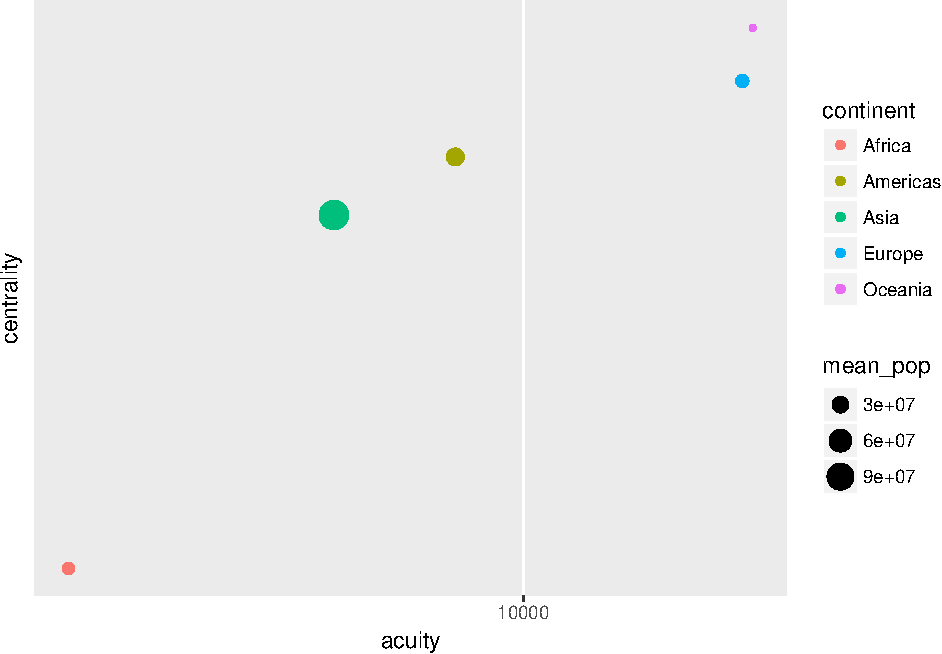
\includegraphics{Flynn_Project_files/figure-latex/unnamed-chunk-2-1.pdf}

\subsection{Schedule}\label{schedule}

Milestone 1: February 14th, 2018 -Objectives Milestone 2: March 15th,
2018 Final Proposal: April 26th, 2018

\section{Results}\label{results}

Results will be discussed with the visual supplementation of network
graphs. This allows the reader to understand concepts that may be
difficult to grasp through text alone.

\section{Discussion}\label{discussion}

Allocating staff resources in an Emergency Department is an ongoing
challenge. How can these results begin to offer solutions to ED staff
and patient management?

What were my primary limitation (both expected and unexpected)?

\section{Conclusion}\label{conclusion}

Did I meet my learning objectives? How would I design a better study
next time?

\section{References}\label{references.unnumbered}

\end{document}


